\section{Experiments and Results}\label{sec:experiments}
After presenting the separation constraints, we test our formulation in a series of experiments to test our rationale and create insights from our proposal. Purposely, we chose three datsets in our experimentation: the \moons dataset (sampling $100$ points, $85$ for training and $15$ for validation), the \texttt{MNIST} dataset as described in LeCun and Cortes. \cite{mnist} and the \texttt{CIFAR-10} dataset devised by Krizhevsky and described in \cite{cifar10}.
\\\\
Inspired by Hasanpour et al. in \cite{simpnet}, we investigate the effect of the constraint formulation on different choices of depth and width, training a family of \emph{rectangular} networks (i.e. networks with fixed layer width $m_k=W$ as presented in our layer function formulation on Equation \ref{eq:layer}) as shown in Table \ref{tab:grids}.
\\\\

\begin{table}[]
\centering
\begin{tabular}{@{}lll@{}}
\toprule
         & Depth & Width \\ \midrule
Moons    & 1-150 & 1-25  \\
MNIST    & 2-64  & 2-8   \\
CIFAR-10 & 1-40  & 10    \\ \bottomrule
\end{tabular}
\caption{}\label{tab:grids}
\end{table}

We the networks were optimized using Adam \cite{adam}. We used a learning rate of $0.01$ for $10000$ epochs and a batch size of $85$ for \moons and a learning rate of $0.001$ for $50$ epochs with a batch size of $1024$ for both \texttt{MNIST} and \texttt{CIFAR-10}. We used an Glorot uniform initialization scheme \cite{Glorot10Initialization} (by default on \texttt{Keras}). We used $\lambda_{MOONS}=10^-4$ $\lambda_{MNIST}=\lambda_{CIFAR}=10^{-8}$ for the Separation Constraints. Our experiments were conducted using \texttt{Keras} \cite{keras} and \texttt{TensorFlow} \cite{tensorflow}, using a random seed with an arbitrary value of $10$. 
\\\\
Graphical summaries of our findings are provided for the reader in all Figures presented in this section. An insidious question that we wish to address throughout our presentation is whether
separation constraints allow us to train \emph{deeper} \emph{rectangular networks}. Our findings are based on a comparison of our proposal to a \emph{baseline} and a \emph{competitor}:  basic \ReLU networks (i.e. the \emph{vanilla} version) and batch-norm as described in \cite{batchnorm}. More specifically, we compare baseline and competitor against three versions of the separating constraints: unit-based separation, (as presented in subsection \ref{subsec:sepUnit}), point-based separation (as detailed in subsection \ref{subsec:sepPoint}) and the combination of both that we denote by \SepUnitPoint. 
\\\\
Figure \ref{fig:moons_grid} shows how training deeper networks requires a layer width-increase, as stated by Hasanpour et al. \cite{simpnet} or Huang et al. \cite{densenet}. This is suggested by beige colored region in \ref{fig:moons_grid_relubn} for \ReLUBN, suggesting a relation of the form
\begin{equation}\label{eq:dependencyWidthDepth}
    D \leq max(\alpha{W} + k, 0) + W_{min}
\end{equation}
where  $w_min>1$. Our experimentation suggests that $W_{min}=3$ However, the relation, notice how the minimum width required to succesfully train networks starts decreasing when , occuring at approximately $D=15$ for \ReLUBN (Figure \ref{fig:moons_grid_relubn}, while for \SepUnitPoint (Figure \ref{fig:moons_grid_up}), accuracy is maintained up to $D=40$ (more than twice the value for \ReLUBN). We identify this linear increase on the width requirements like the use of the width-increase strategy, which hints that \SepPoint is able to avoiding to use it further than \ReLUBN.

\\\\
All of our versions of separation constraints outperform consistently both \ReLU and \ReLUBN, as we can see in Table \ref{tab:moons}. Indeed, in Figures \ref{fig:moons_grid_u}, \ref{fig:moons_grid_p} and \ref{fig:moons_grid_up} we see how the use of the separation constraints enable to use deeper networks with the same width. 
\\\\
More so, Figures \ref{fig:moons_grid_u},\ref{fig:moons_grid_p} and \ref{fig:moons_grid_up} show us that the minimum width required to train successfully (with a $95+\%$ accuracy) can be done  starting decreasing from $3$ units per layer approximately at depth $15$ for \ReLUBN (Figure \ref{fig:moons_grid_relubn}, whereas \SepUnitPoint (Figure \ref{fig:moons_grid_up}) is able to maintain up to $40$ layers deep, more than twice. We identify this linear increase on the width requirements like the use of the width-increase strategy, which hints that \SepPoint is able to avoiding to use it further than \ReLUBN.
\\\\
Regarding the differences among Separation constraint variations, \SepUnit is the one which is able to train deeper networks (Figure \ref{fig:moons_grid_u}, although at lower accuracy and showing the same linear degradation after layer $14$ as \ReLUBN (Figure \ref{fig:moons_grid_relubn}), like an improved but not perfect version of it. \SepPoint (Figure \ref{fig:moons_grid_p}) in the other hand it is able to maintain the minimum width longer than both \ReLUBN and \SepUnit, but it suffers from the same abrupt breakdown as \ReLU but with an small successful area around width $4$. Finally, the combination of both, \SepUnitPoint (Figure \ref{fig:moons_grid_up}) allows to improve both the accuracy and minimum width figures of both \SepUnit and \SepPoint, hinting that their effect during the training is enhanced by each other.
\\\\
The same effect seen with a fully-connected network applied to a toy dataset such as \moons can be seen in other common vision datasets such as MNIST \cite{mnist} or CIFAR-10 \cite{cifar10} when using convolutional networks. Figure \ref{fig:mnist_grid} shows the same behaviour from the \moons dataset (Figure\ref{fig:moons_grid}), where \ReLU breaks down after few layers, \ReLUBN holds it better but eventually starts degradating whereas \SepUnitPoint is able to work equally well disregarding the depth used. In the case of CIFAR-10, the results (Table \ref{tab:cifar10}) show how with few layers \ReLU and \ReLUBN match or improve \SepUnitPoint but after adding some layers it gets even until \SepUnitPoint surpasses them.


\begin{figure*}
  \centering
    \begin{subfigure}[b]{0.3\textwidth}
        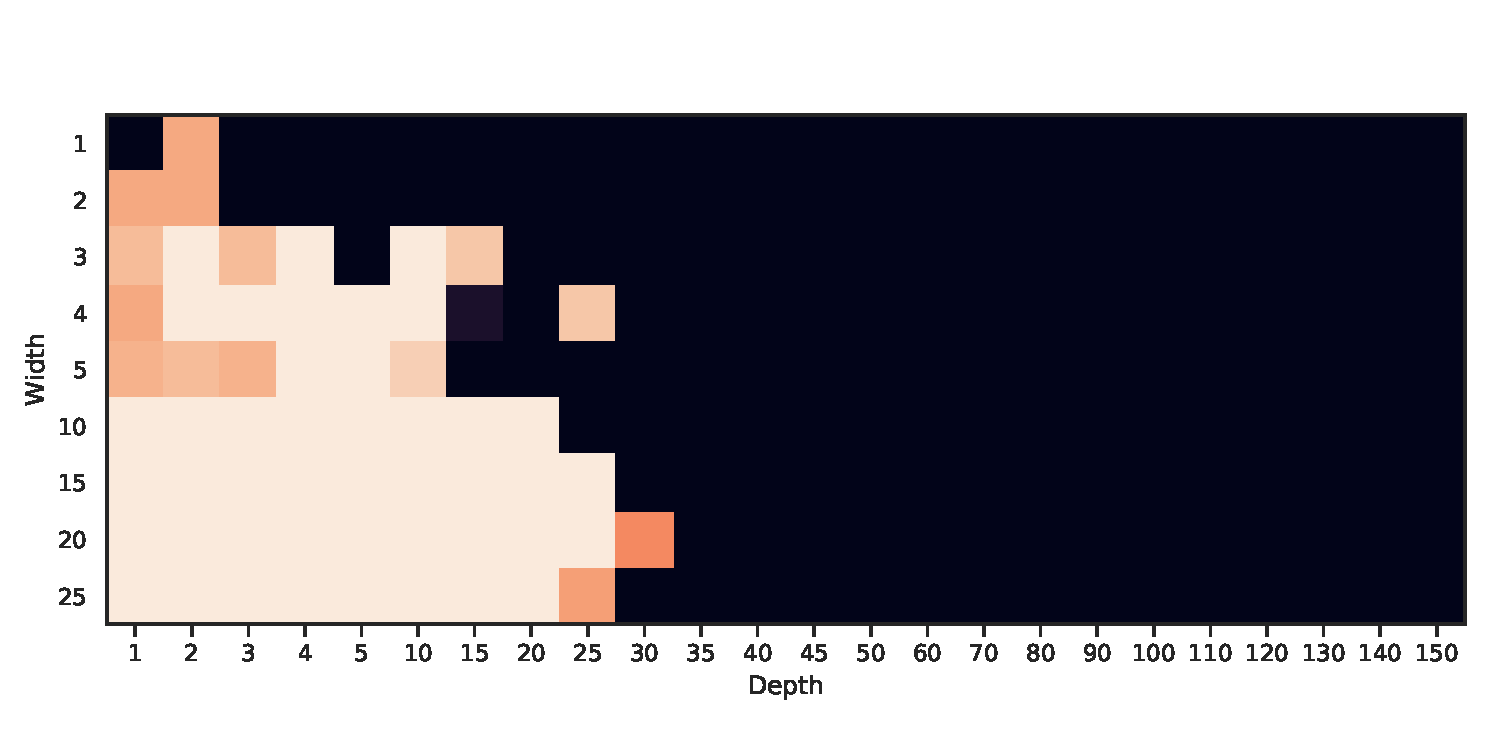
\includegraphics[width=\textwidth]{img/moons_grid/acc-relu.pdf}
        \caption{\ReLU training}
        \label{fig:moons_grid_relu}
    \end{subfigure}
    ~ %add desired spacing between images, e. g. ~, \quad, \qquad, \hfill etc. 
      %(or a blank line to force the subfigure onto a new line)
    \centering
    \begin{subfigure}[b]{0.3\textwidth}
        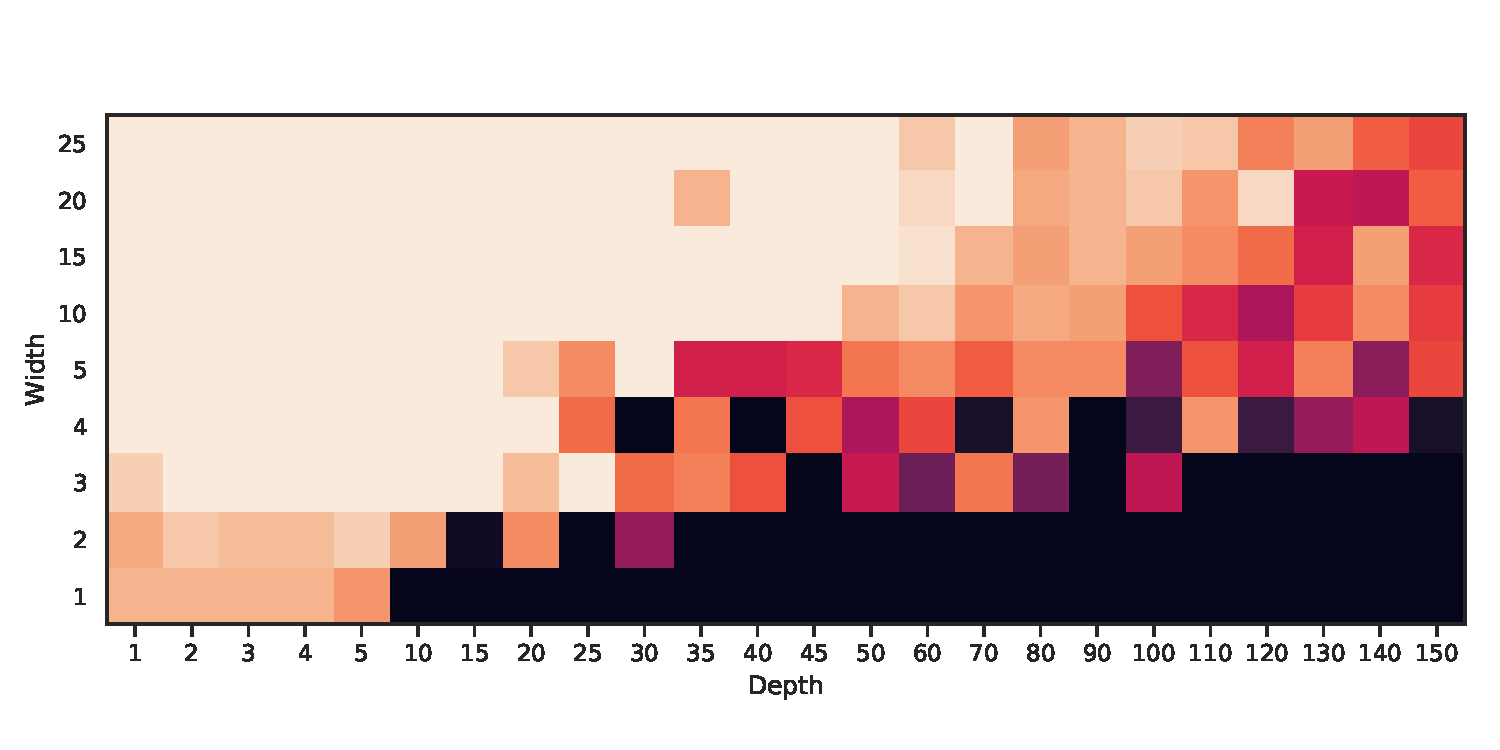
\includegraphics[width=\textwidth]{img/moons_grid/acc-relu-bn.pdf}
        \caption{\ReLUBN training}
        \label{fig:moons_grid_relubn}
    \end{subfigure}
    ~ %add desired spacing between images, e. g. ~, \quad, \qquad, \hfill etc. 
      %(or a blank line to force the subfigure onto a new line)
    \centering
    \begin{subfigure}[b]{0.3\textwidth}
        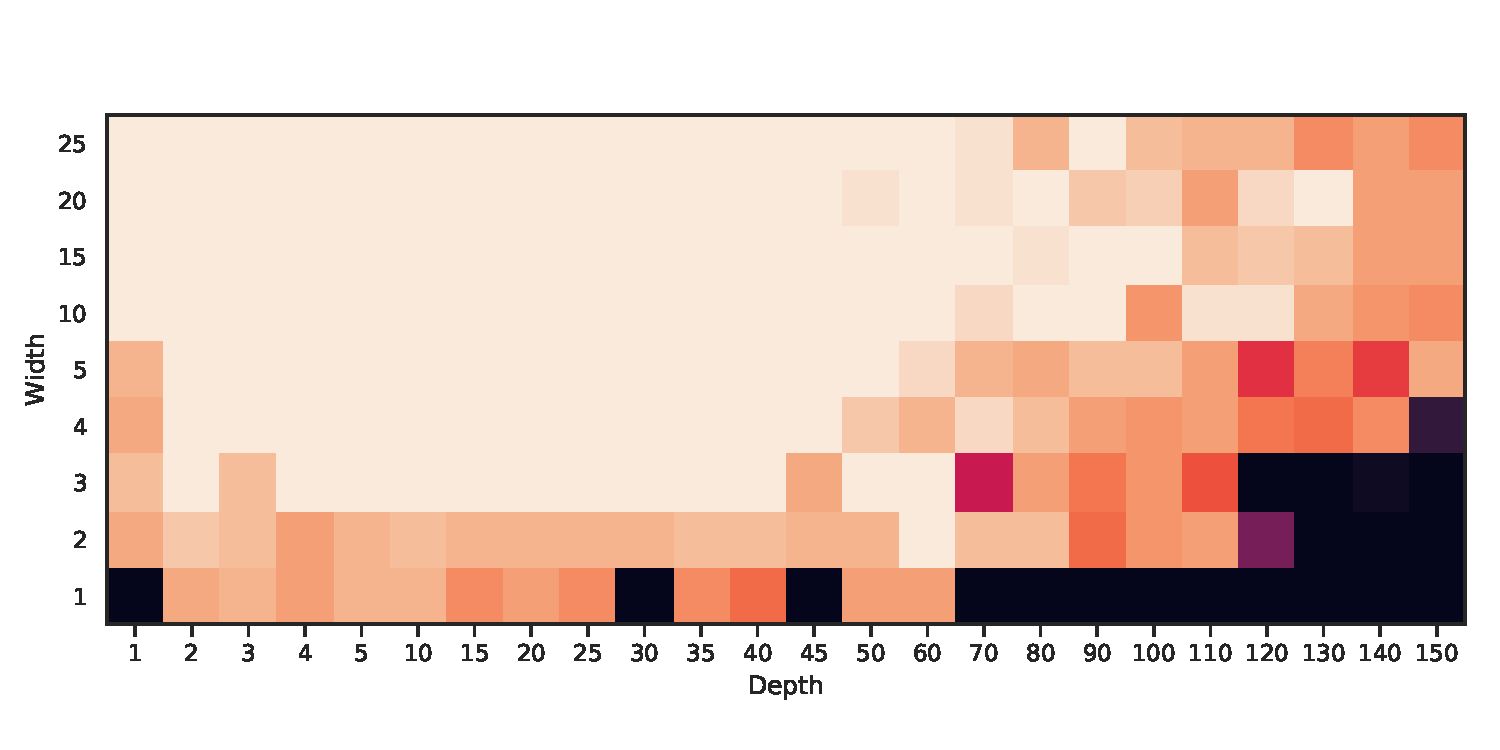
\includegraphics[width=\textwidth]{img/moons_grid/acc-sep-up-0-0001.pdf}
        \caption{\SepUnitPoint training}
        \label{fig:moons_grid_up}
    \end{subfigure}
    ~ %add desired spacing between images, e. g. ~, \quad, \qquad, \hfill etc. 
      %(or a blank line to force the subfigure onto a new line)
    \\
    \begin{subfigure}[b]{0.3\textwidth}
        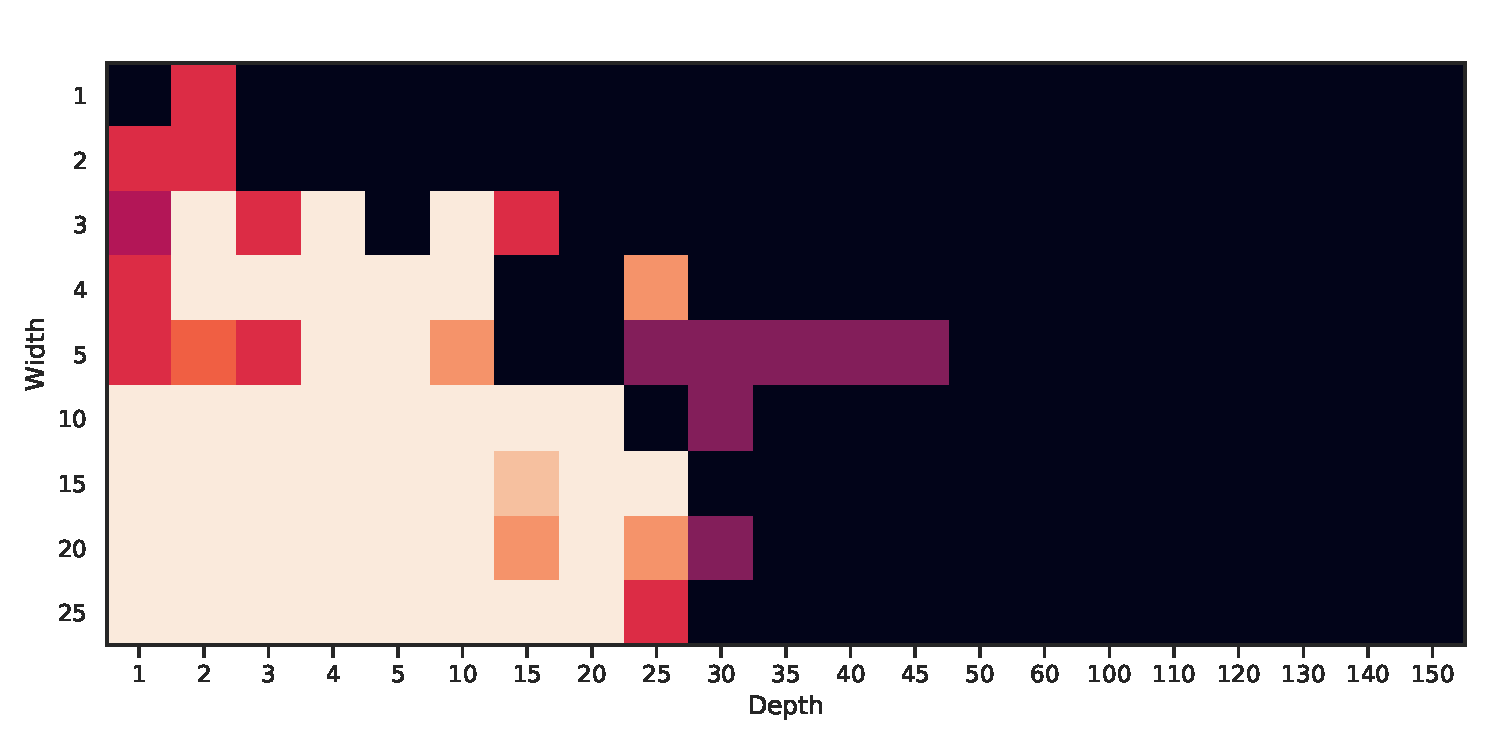
\includegraphics[width=\textwidth]{img/moons_grid/val-acc-relu.pdf}
        \caption{\ReLU validation}
        \label{fig:moons_grid_relu}
    \end{subfigure}
    ~ %add desired spacing between images, e. g. ~, \quad, \qquad, \hfill etc. 
      %(or a blank line to force the subfigure onto a new line)
    \centering
    \begin{subfigure}[b]{0.3\textwidth}
        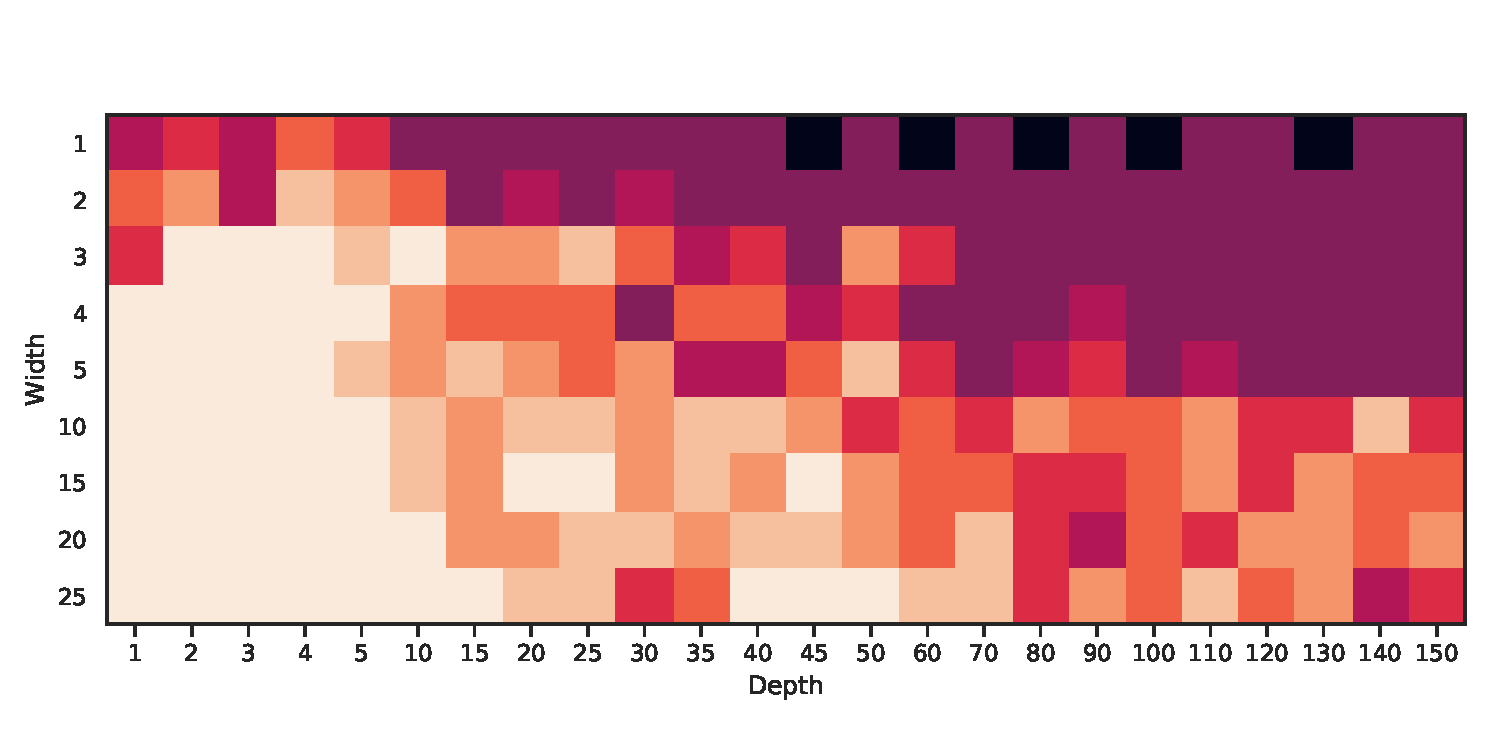
\includegraphics[width=\textwidth]{img/moons_grid/val-acc-relu-bn.pdf}
        \caption{\ReLUBN validation}
        \label{fig:moons_grid_relubn}
    \end{subfigure}
    ~ %add desired spacing between images, e. g. ~, \quad, \qquad, \hfill etc. 
      %(or a blank line to force the subfigure onto a new line)
    \centering
    \begin{subfigure}[b]{0.3\textwidth}
        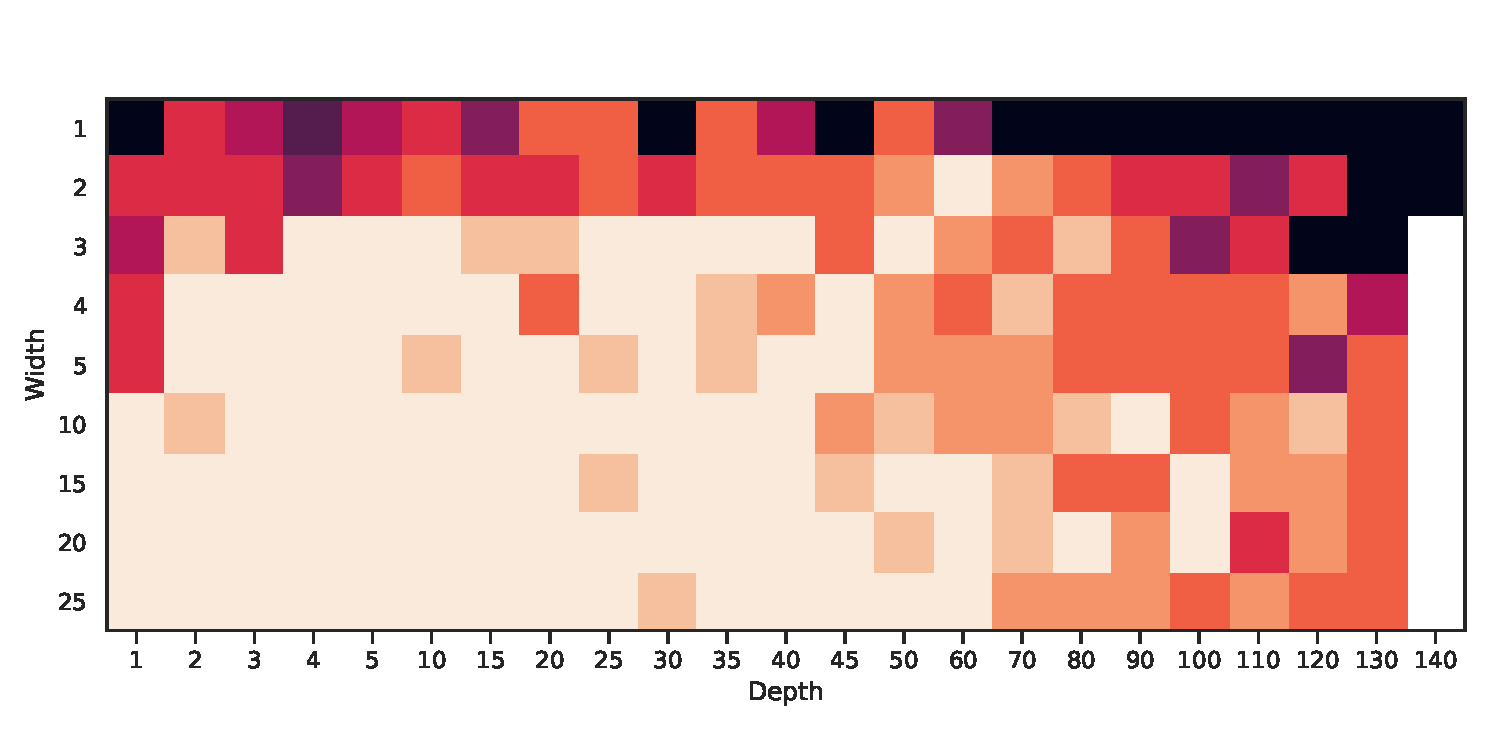
\includegraphics[width=\textwidth]{img/moons_grid/val-acc-sep-up-0-0001.pdf}
        \caption{\SepUnitPoint validation}
        \label{fig:moons_grid_up}
    \end{subfigure}
    ~ %add desired spacing between images, e. g. ~, \quad, \qquad, \hfill etc. 
      %(or a blank line to force the subfigure onto a new line)
      \\
    \begin{subfigure}[b]{0.3\textwidth}
        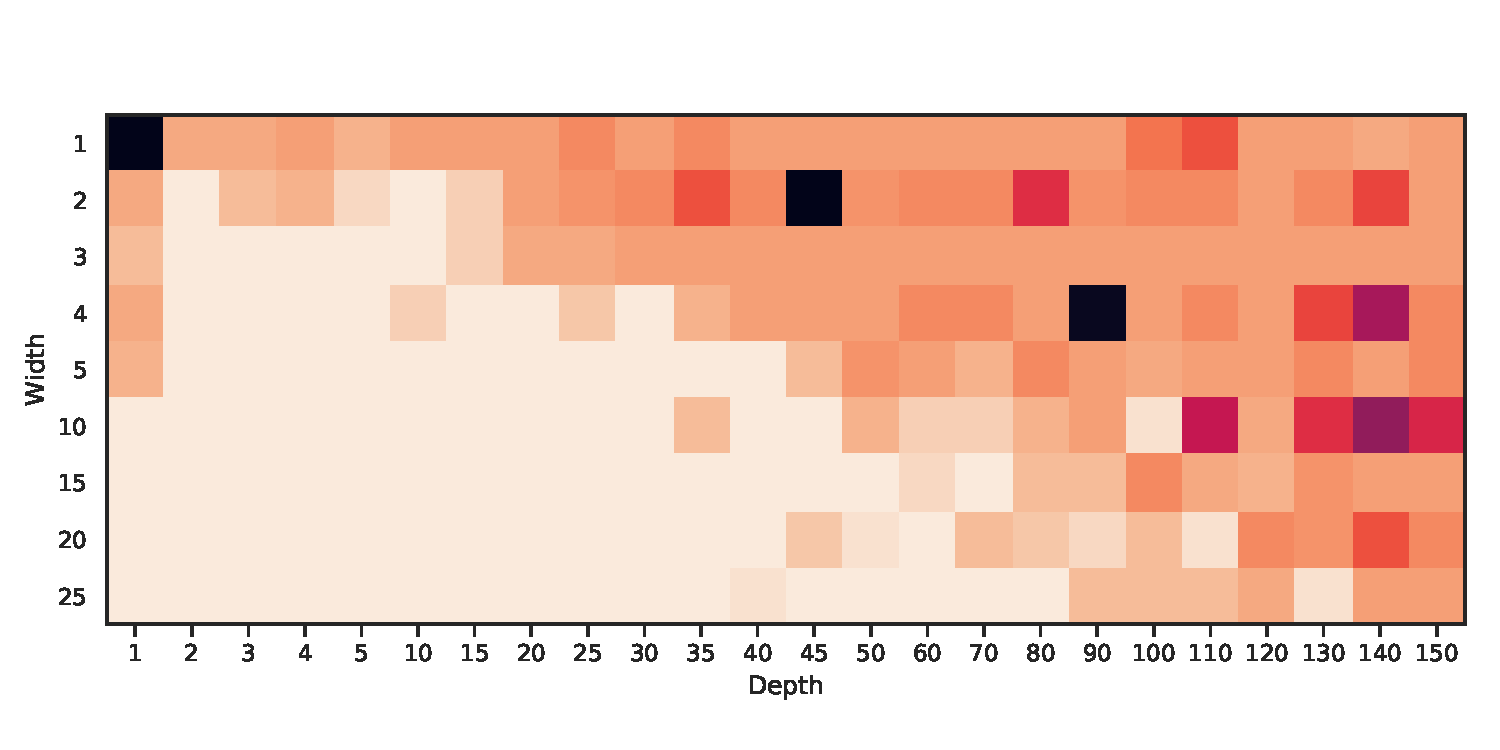
\includegraphics[width=\textwidth]{img/moons_grid/acc-sep-u-0-0001.pdf}
        \caption{\SepUnit training}
        \label{fig:moons_grid_u}
    \end{subfigure}
    ~ %add desired spacing between images, e. g. ~, \quad, \qquad, \hfill etc. 
      %(or a blank line to force the subfigure onto a new line)
    \centering
    \begin{subfigure}[b]{0.3\textwidth}
        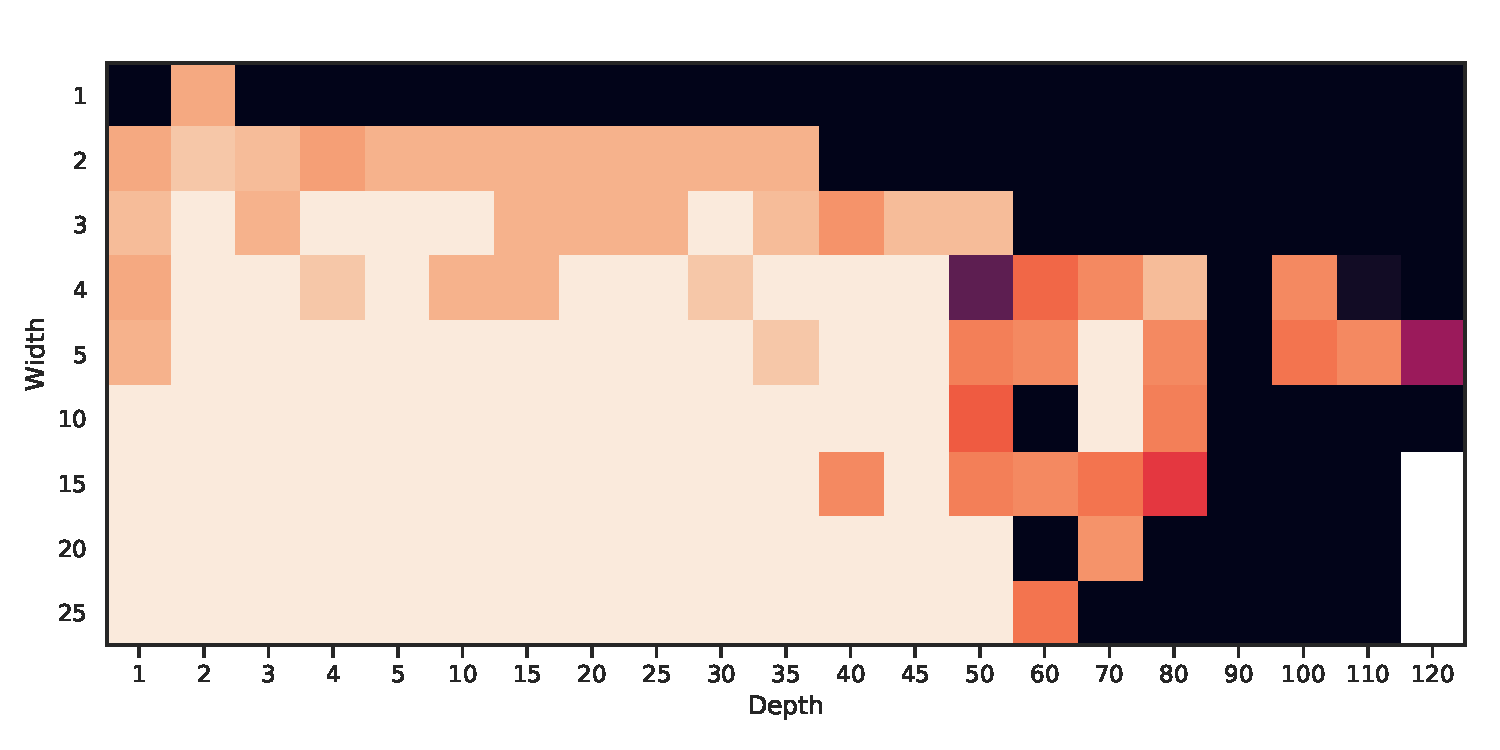
\includegraphics[width=\textwidth]{img/moons_grid/acc-sep-p-0-0001.pdf}
        \caption{\SepPoint training}
        \label{fig:moons_grid_p}
    \end{subfigure}
    ~ %add desired spacing between images, e. g. ~, \quad, \qquad, \hfill etc. 
      %(or a blank line to force the subfigure onto a new line)
    \\
    \begin{subfigure}[b]{0.3\textwidth}
        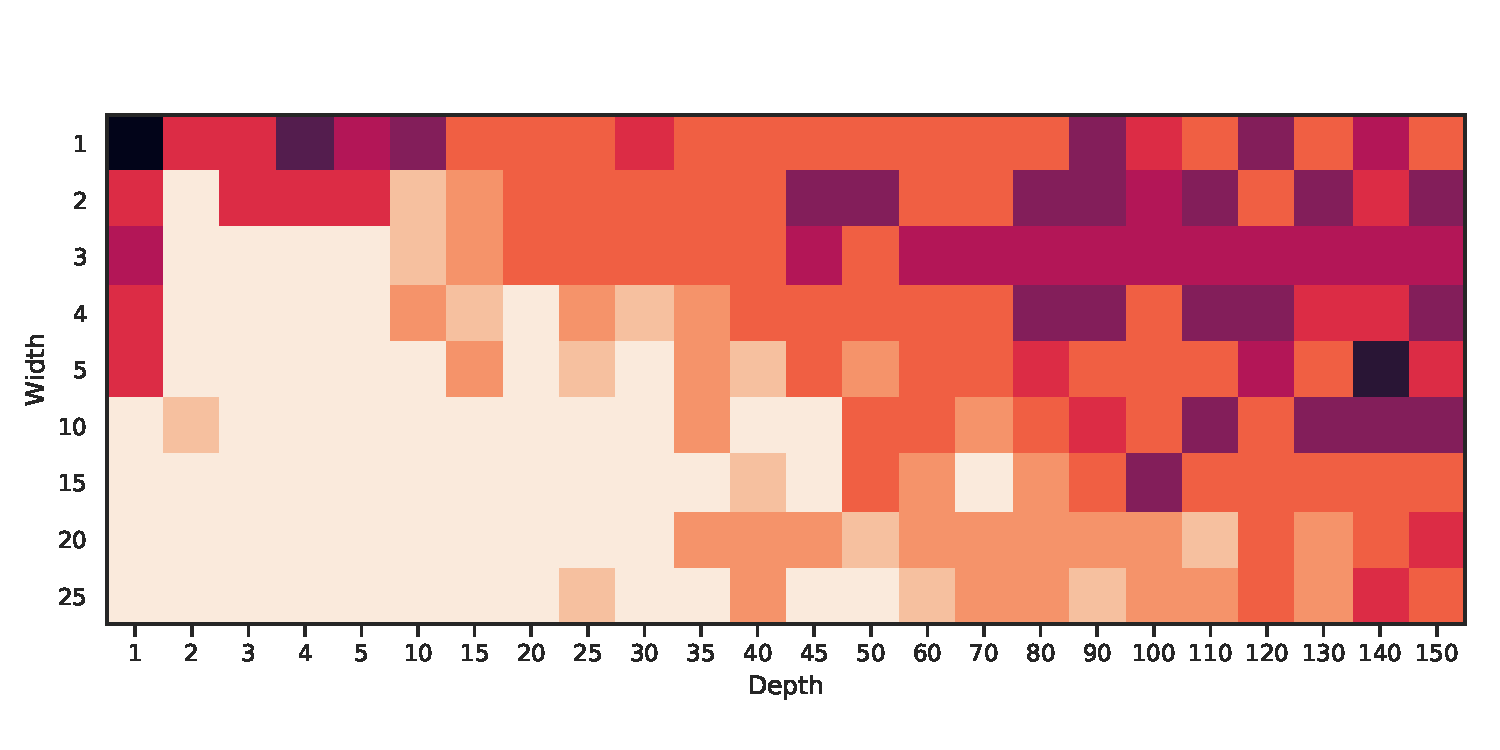
\includegraphics[width=\textwidth]{img/moons_grid/val-acc-sep-u-0-0001.pdf}
        \caption{\SepUnit validation}
        \label{fig:moons_grid_u}
    \end{subfigure}
    ~ %add desired spacing between images, e. g. ~, \quad, \qquad, \hfill etc. 
      %(or a blank line to force the subfigure onto a new line)
    \centering
    \begin{subfigure}[b]{0.3\textwidth}
        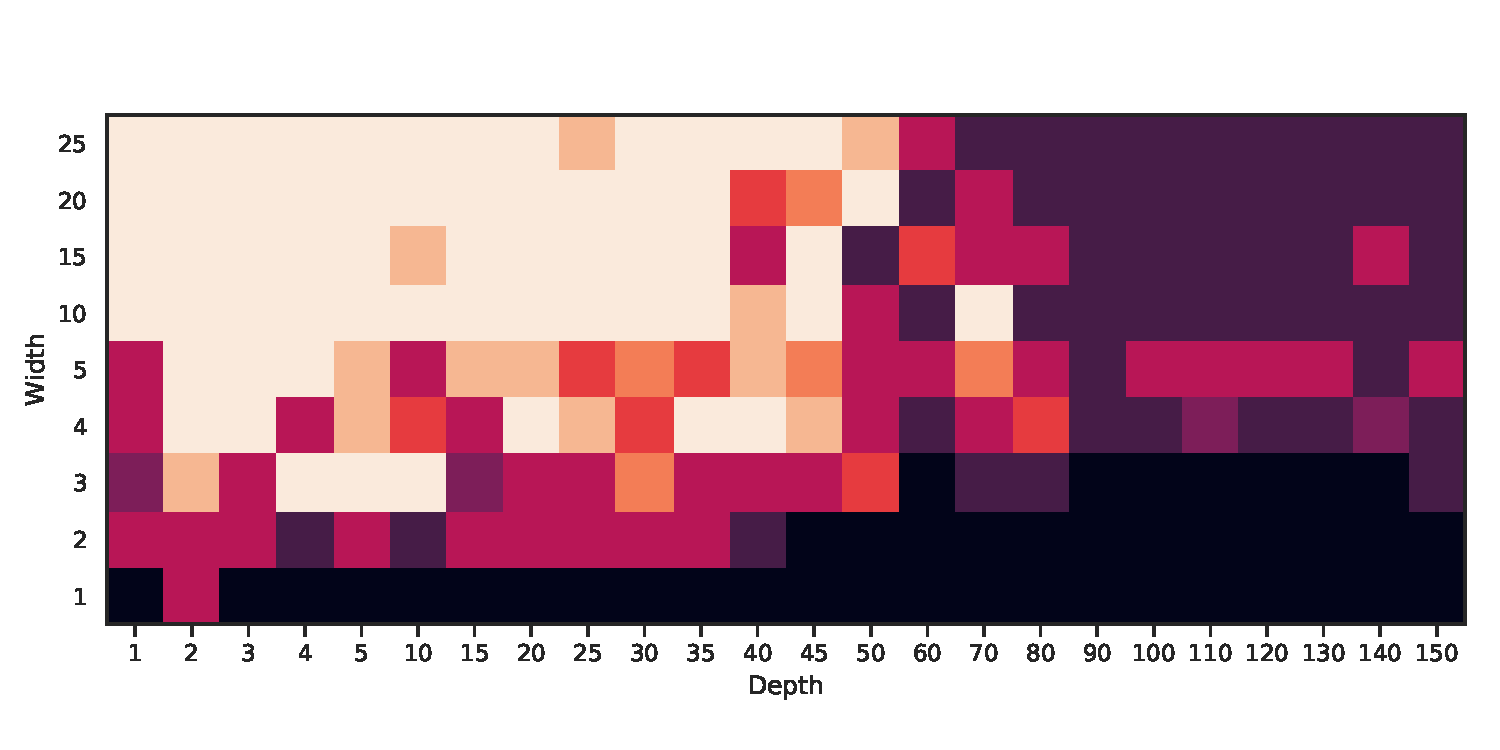
\includegraphics[width=\textwidth]{img/moons_grid/val-acc-sep-p-0-0001.pdf}
        \caption{\SepPoint validation}
        \label{fig:moons_grid_p}
    \end{subfigure}
    ~ %add desired spacing between images, e. g. ~, \quad, \qquad, \hfill etc. 
      %(or a blank line to force the subfigure onto a new line)
    
    
  \caption{Depth vs Width accuracy plot a for rectangular network using a grid (width from $2$ to $25$ and depth from $2$ to $150$),  trained using a Adam learning rate of $0.01$ in the \moons dataset. The color show the accuracy attained of each of the combinations of width and depth, the clearer the better. Notice how \ReLU, Figure \ref{fig:moons_grid_relu}, fails with networks deeper than 30 layers. In other hand, \ReLUBN, Figure \ref{fig:moons_grid_relubn}, manages to work until 70 layers deep. \SepUnitPoint,  Figure \ref{fig:moons_grid_up}, works significantly better than both, up to 120 layers. Notice how all the methods suffer from degradation from depth, which is partially alleviated by the use of greater width. This is consistent with \cite{simpnet} and \cite{densenet}. However, \SepUnitPoint is able to delay the apparition of the issue. This is especially visible when the number of units is small (from $2$ to $5$) where \ReLUBN fails to work whereas \SepUnitPoint does not. Regarding to the role of the constraint on its success, we find that \SepUnit, Figure \ref{fig:moons_grid_u}, allows the network to grow deeper, yet the accuracy can be lower following the linear decrease with the inverse of the width, which we blame on the inability of the \SepUnit constraint to address the \emph{dead point} issue. In the other hand, \SepPoint, Figure \ref{fig:moons_grid_p}, seems to perform well up to 50 layers, but it breaks down afterwards. Finally, \SepLayer , Figure \ref{fig:moons_grid_l} seems to suffer if the width is too large, performing well up to 70 layers.}
  \label{fig:moons_grid} 
\end{figure*}


\begin{figure*}
  \centering
    \begin{subfigure}[b]{0.3\textwidth}
        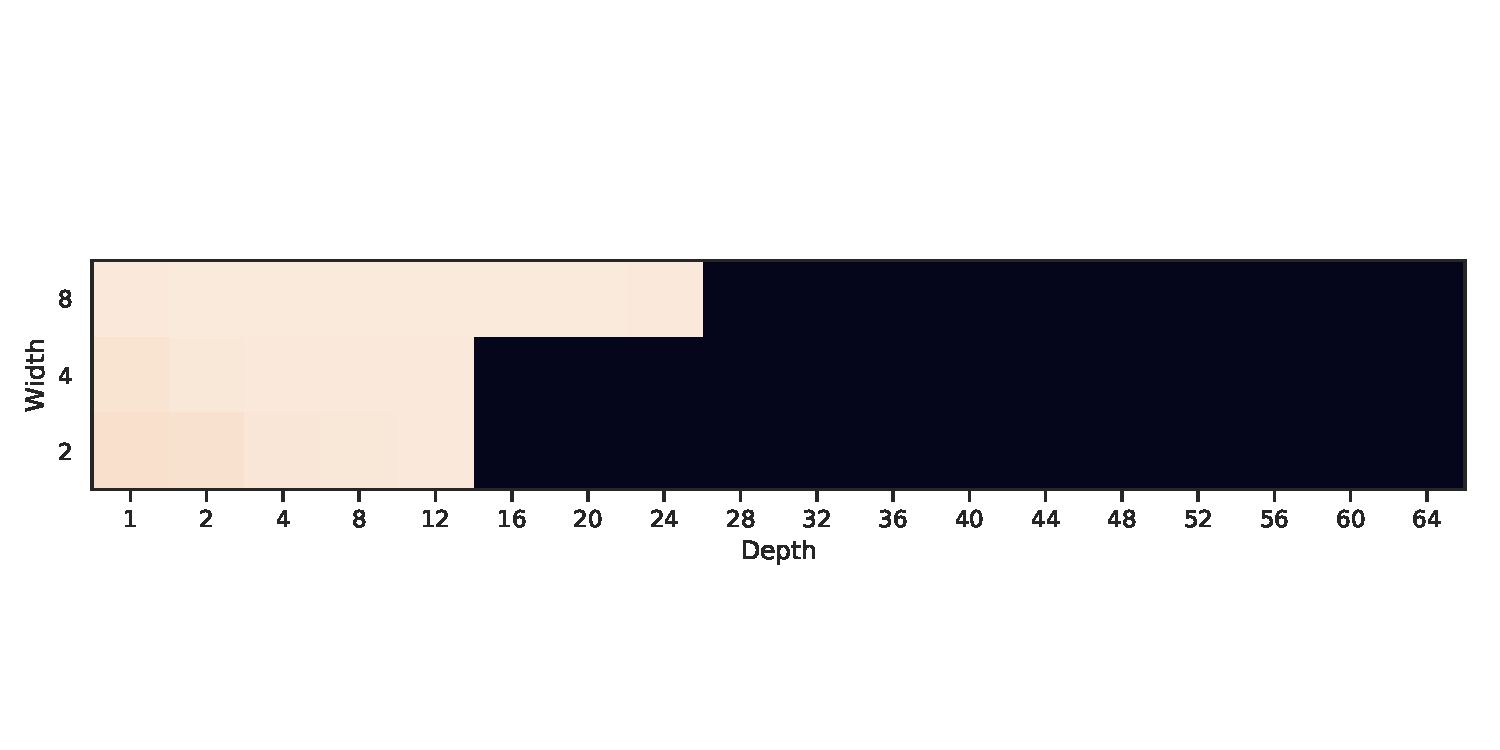
\includegraphics[width=\textwidth]{img/mnist_grid/acc-relu-ks-3x3-bs-1024.pdf}
        \caption{\ReLU}
        \label{fig:mnist_grid_relu}
    \end{subfigure}
    ~ %add desired spacing between images, e. g. ~, \quad, \qquad, \hfill etc. 
      %(or a blank line to force the subfigure onto a new line)
    \centering
    \begin{subfigure}[b]{0.3\textwidth}
        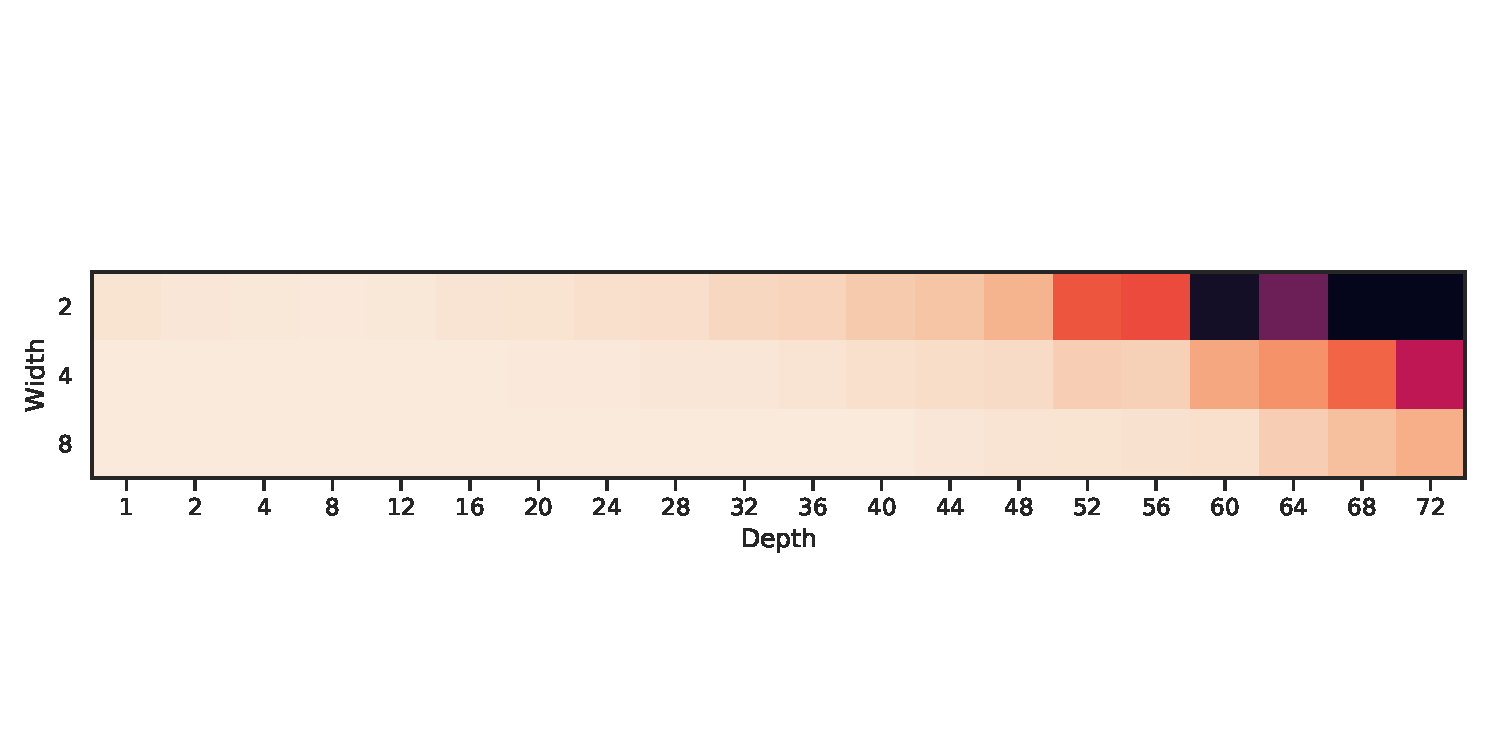
\includegraphics[width=\textwidth]{img/mnist_grid/acc-relu-bn-ks-3x3-bs-1024.pdf}
        \caption{\ReLUBN}
        \label{fig:mnist_grid_relubn}
    \end{subfigure}
    ~ %add desired spacing between images, e. g. ~, \quad, \qquad, \hfill etc. 
      %(or a blank line to force the subfigure onto a new line)
    \centering
    \begin{subfigure}[b]{0.3\textwidth}
        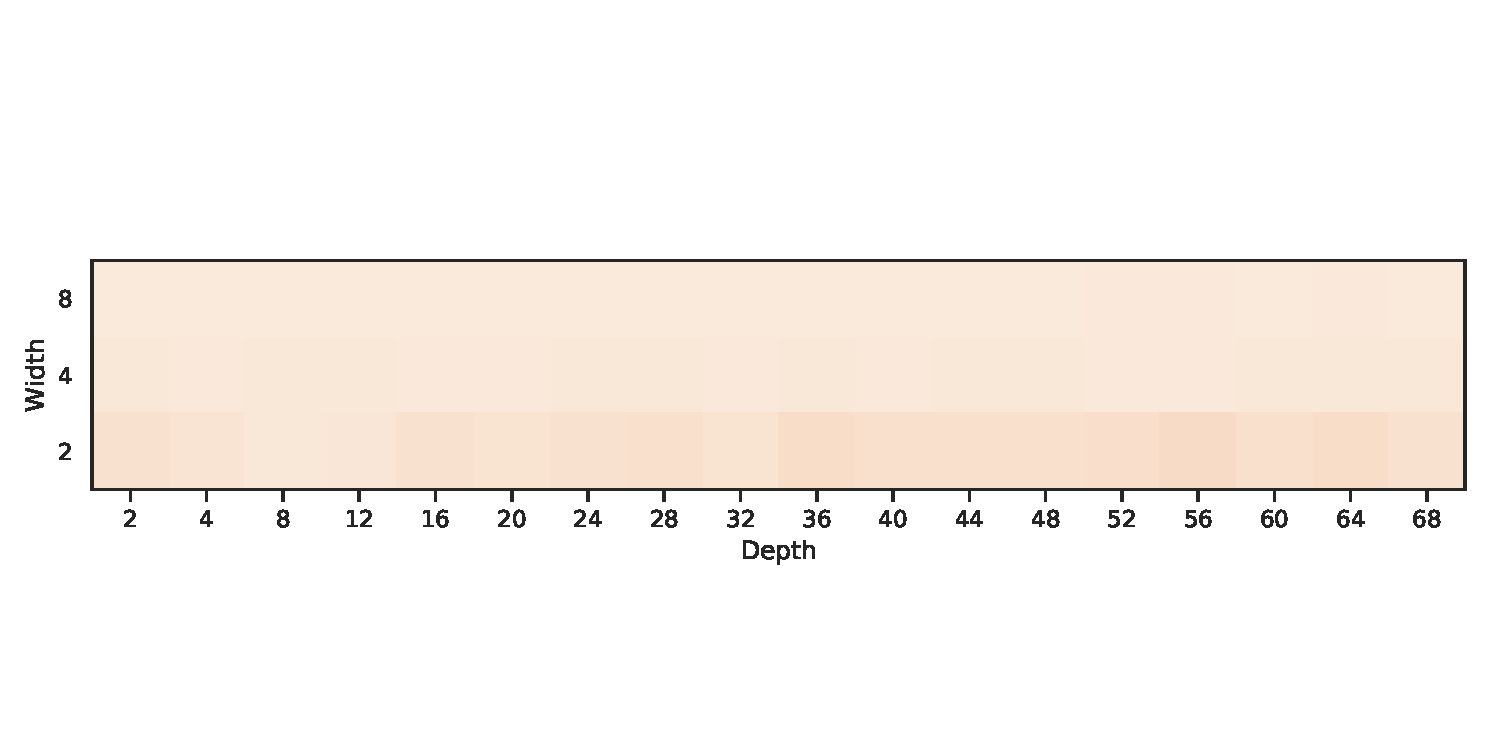
\includegraphics[width=\textwidth]{img/mnist_grid/acc-sep-up-1e-08-ks-3x3-bs-1024.pdf}
        \caption{\SepUnitPoint}
        \label{fig:mnist_grid_up}
    \end{subfigure}
    ~ %add desired spacing between images, e. g. ~, \quad, \qquad, \hfill etc. 
      %(or a blank line to force the subfigure onto a new line)
    
  \caption{Depth vs Width accuracy plot a for rectangular network using a grid (width from $2$ to $25$ and depth from $2$ to $150$),  trained using a Adam learning rate of $0.01$ in the MNIST dataset. The color show the accuracy attained of each of the combinations of width and depth, the clearer the better. Notice how \ReLU, Figure \ref{fig:mnist_grid_relu}, fails with networks deeper than 30 layers. In other hand, \ReLUBN, Figure \ref{fig:mnist_grid_relubn}, manages to work until 70 layers deep. \SepUnitPoint,  Figure \ref{fig:mnist_grid_up}, works significantly better than both, up to 120 layers. Notice how all the methods suffer from degradation from depth, which is partially alleviated by the use of greater width. This is consistent with \cite{simpnet} and \cite{densenet}. However, \SepUnitPoint is able to delay the apparition of the issue. This is especially visible when the number of units is small (from $2$ to $5$) where \ReLUBN fails to work whereas \SepUnitPoint does not.}
  \label{fig:mnist_grid} 
\end{figure*}



\begin{table*}
\begin{tabular}{llrrrrr}
\toprule
                    &    &       2  &       10 &       25 &       30 &       40 \\
\midrule
relu ks 3x3 & 10 &  0.72142 &  0.82748 &  0.09906 &  0.09880 &  0.09810 \\
relu-bn ks 3x3 & 10 &  0.90580 &  0.81764 &  0.70496 &  0.66718 &  0.59642 \\
Sep-UP 1e-08 ks 3x3 & 10 &  0.69264 &  0.79044 &  0.74344 &  0.70452 &  0.68416 \\
\bottomrule
\end{tabular}

\\
\begin{tabular}{llrrrrr}
\toprule
                    &    &      2  &      10 &      25 &      30 &      40 \\
\midrule
relu ks 3x3 & 10 &  0.5958 &  0.6052 &  0.1000 &  0.1000 &  0.1000 \\
relu-bn ks 3x3 & 10 &  0.5682 &  0.5385 &  0.5414 &  0.5328 &  0.4512 \\
Sep-UP 1e-08 ks 3x3 & 10 &  0.5874 &  0.5703 &  0.5353 &  0.5300 &  0.5320 \\
\bottomrule
\end{tabular}

\caption{}\label{tab:cifar10}
\end{table*}